%%----------------------------------------------------------------------------
%% Presentatie HoGent Bedrijf en Organisatie
%%----------------------------------------------------------------------------
%% Auteur: Bert Van Vreckem [bert.vanvreckem@hogent.be]

\documentclass{beamer}

%==============================================================================
% Aanloop
%==============================================================================

%---------- Packages ----------------------------------------------------------

\usepackage{graphicx,multicol}
\usepackage{comment,enumerate,hyperref}
\usepackage{amsmath,amsfonts,amssymb}
\usepackage{tikz}
\usepackage[english]{babel}
\usepackage[utf8]{inputenc}
\usepackage{multirow}
\usepackage{eurosym}
\usepackage{listings}
\usepackage[T1]{fontenc}
\usepackage{lmodern}
\usepackage{textcomp}
\usepackage{framed}
\usepackage{wrapfig}

%---------- Configuratie ------------------------------------------------------

\usetikzlibrary{arrows,shapes,backgrounds,positioning,shadows}

\usetheme{hogent}

%---------- Commando-definities -----------------------------------------------

\newcommand{\tabitem}{~~\llap{\textbullet}~~}

%---------- Info over de presentatie ------------------------------------------

\title[Intro]{Quick Workshop Android}
\author{Dr. Jens Buysse }
\date{2014-2015}

%==============================================================================
% Inhoud presentatie
%==============================================================================

\begin{document}

%---------- Front matter ------------------------------------------------------

% Dia met het HoGent logo
\HoGentLogo

% Titeldia met faculteitslogo
\titleframe

%---------- Inhoud ------------------------------------------------------------

\section{Welcome to Mobile: Android}
\sectionframe

\begin{frame}
	\frametitle{Hello Android}
	I've come up with a set of rules that describe our reactions to
technologies:
\begin{enumerate}
	\item Anything that is in the world when you're born is normal and ordinary and is just a natural part of the way the world works.
	\item Anything that's invented between when you're fifteen and thirty-five is new and exciting and revolutionary and you can probably get a career in it.
	\item Anything invented after you're thirty-five is against the natural order of things.
\end{enumerate}
\begin{flushright}

\end{flushright}
-- Douglas Adams, author of \textsl{Hithhiker's Guide to the Galaxy}
\end{frame}

\begin{frame}
	\frametitle{Mobile Development}
	\begin{columns}
		\begin{column}{0.3 \textwidth}
		\pause
		\begin{figure}
			\centering
				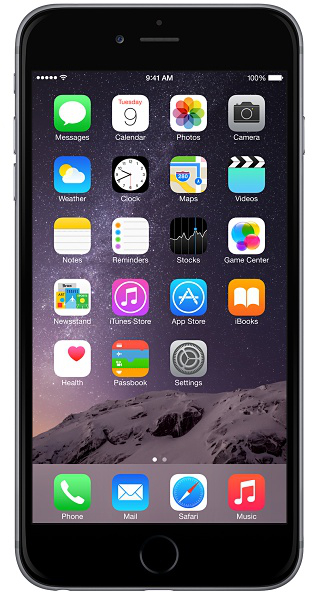
\includegraphics[width=1.00\textwidth]{img/iphone.jpg}
			\label{fig:iphone}
		\end{figure}
		
		\end{column}
		\begin{column}{0.3 \textwidth}
		\pause
			\begin{figure}
			\centering
				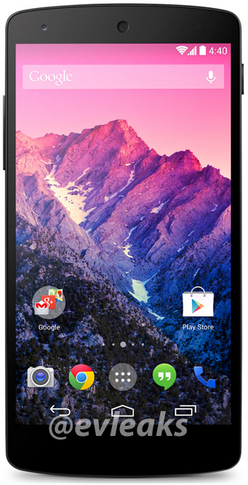
\includegraphics[width=1.00\textwidth]{img/nexus.png}
			\label{fig:iphone}
		\end{figure}
		\end{column}
		\begin{column}{0.3 \textwidth}
		\pause
			\begin{figure}
			\centering
				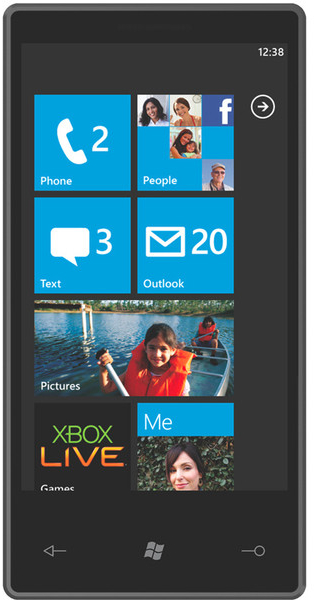
\includegraphics[width=1.00\textwidth]{img/windowsPhone.jpg}
			\label{fig:iphone}
		\end{figure}
		\end{column}
	\end{columns}
\end{frame}


{
\usebackgroundtemplate{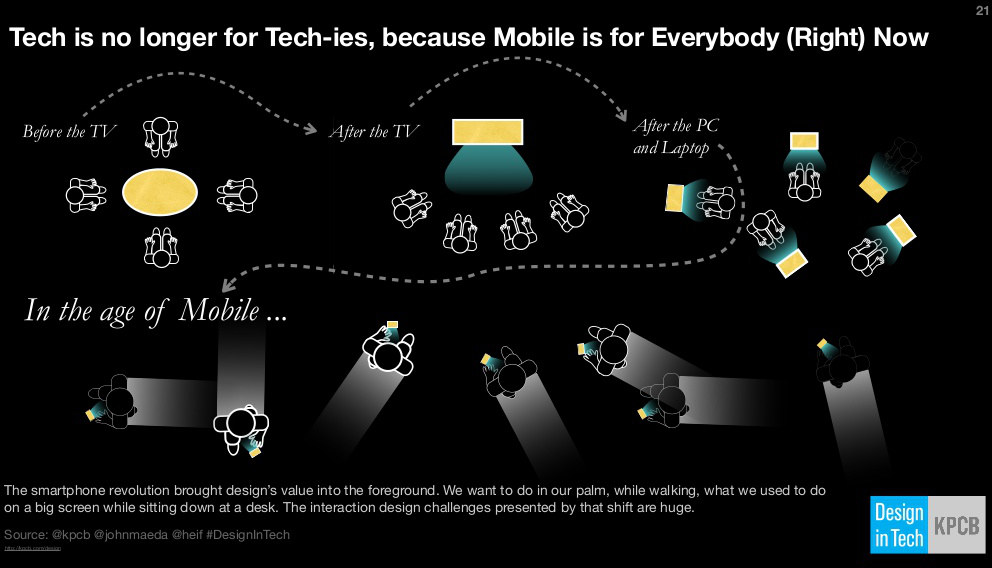
\includegraphics[height=\paperheight,width=\paperwidth]{img/timeLineMobile.jpg}}
\setbeamertemplate{navigation symbols}{}
\begin{frame}[plain]
\end{frame}
}

\begin{frame}
	\frametitle{What is Android}
	
	\begin{figure}
		\centering
			
\includegraphics[width=0.3 \textwidth]{img/androidlogo.png}
		\label{fig:androidlogo}
	\end{figure}
	
	Android is a ecosystem consisting of the following components:
	
	\begin{enumerate}
		\item A free, open source, operating system for embedded devices \pause
		\item An open source development platform to create mobile applications \pause
		\item Devices, specifically mobile devices, which run the mobile Android OS and the applications made for it
	\end{enumerate}
	 
	See \url{http://developer.android.com/training}
	
\end{frame}

{
	\usebackgroundtemplate{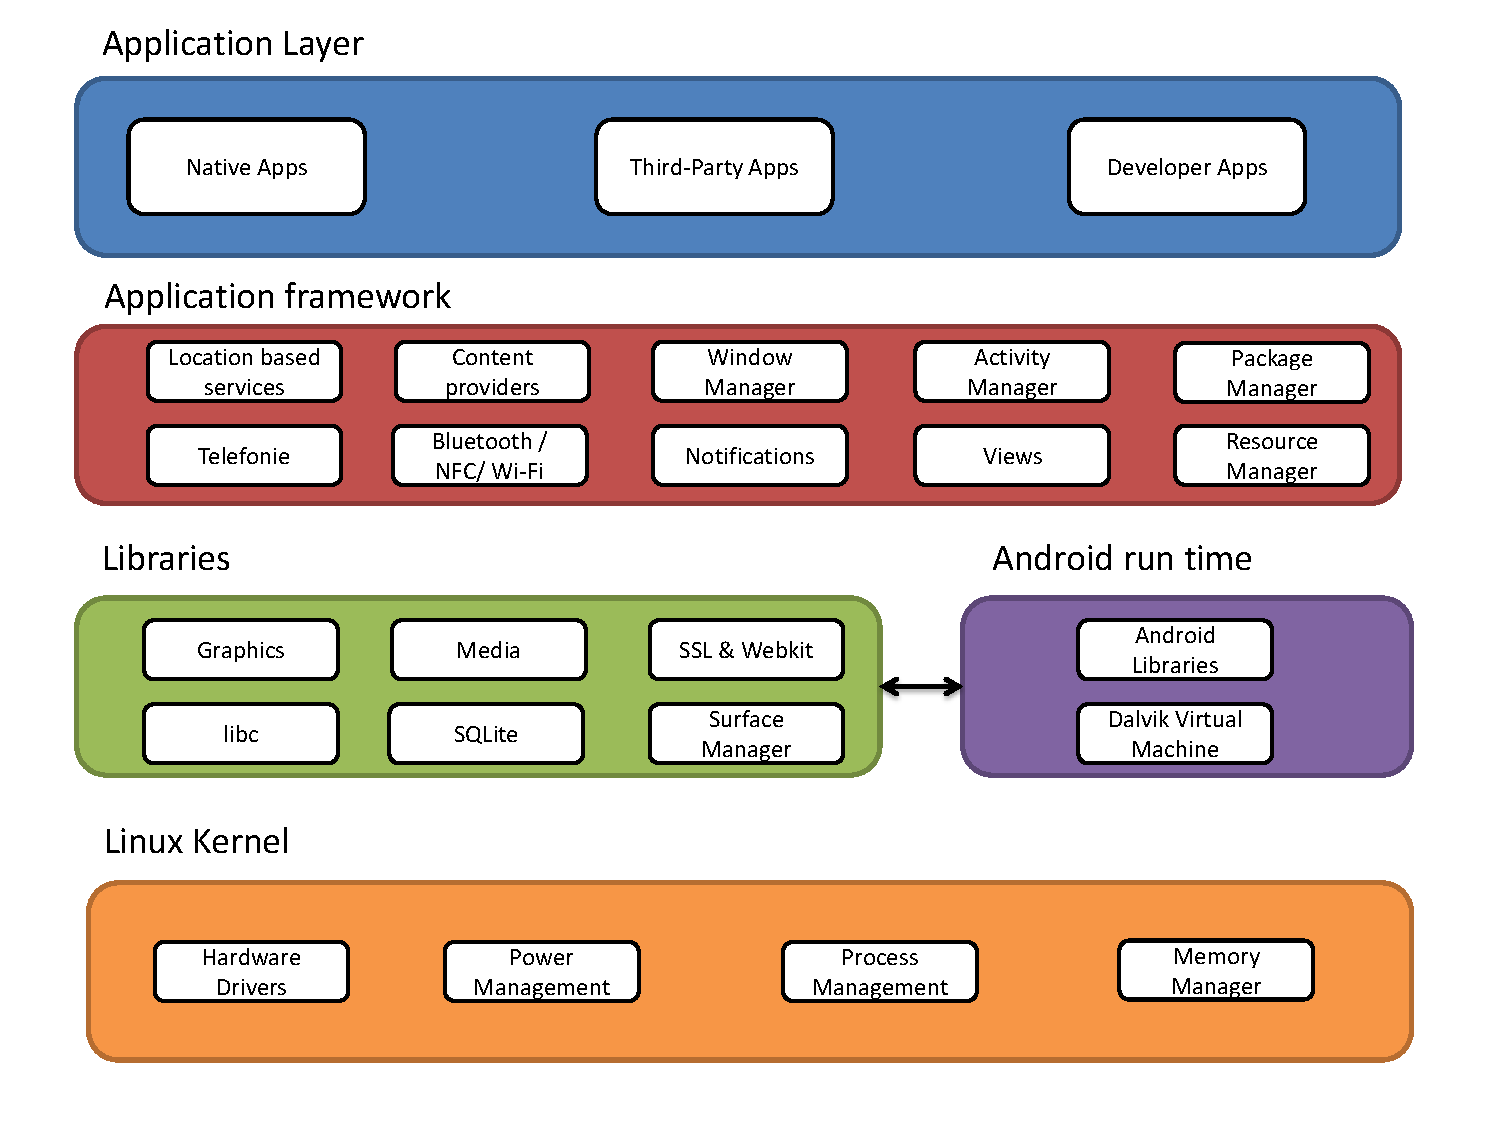
\includegraphics[height=\paperheight,width=\paperwidth]{img/androidstack.pdf}}
	\setbeamertemplate{navigation symbols}{}
	\begin{frame}[plain]
	\end{frame}
}
	
\begin{frame}
\frametitle{Linux Kernel}
Core services:
\begin{itemize}
\item Hardware drivers
\item Process and Memory management
\item Security and Power Management
\end{itemize}
De Kernel is a layer of abstraction between hardware and rest of Software Stack

\begin{figure}[b]
	\centering
		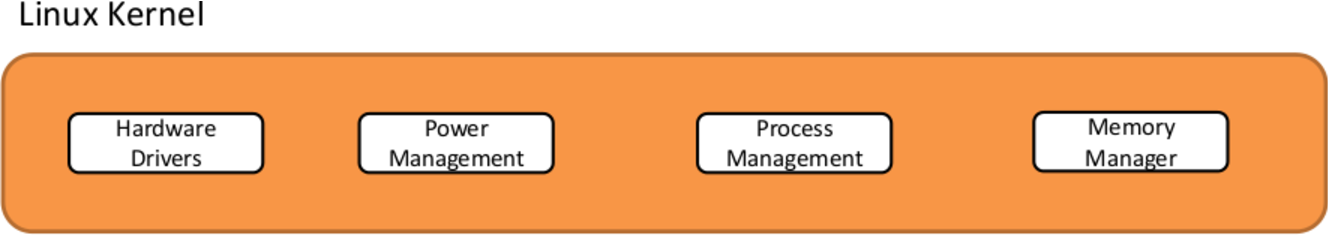
\includegraphics[width=\textwidth]{img/kernel.pdf}
	\label{fig:kernel}
\end{figure}

\end{frame}

\begin{frame}
\frametitle{Libraries}
\begin{itemize}
\item Media Library
\item Graphical libraries 
\item SQLLite for database support
\item \dots
\end{itemize}

\begin{figure}[b]
	\centering
		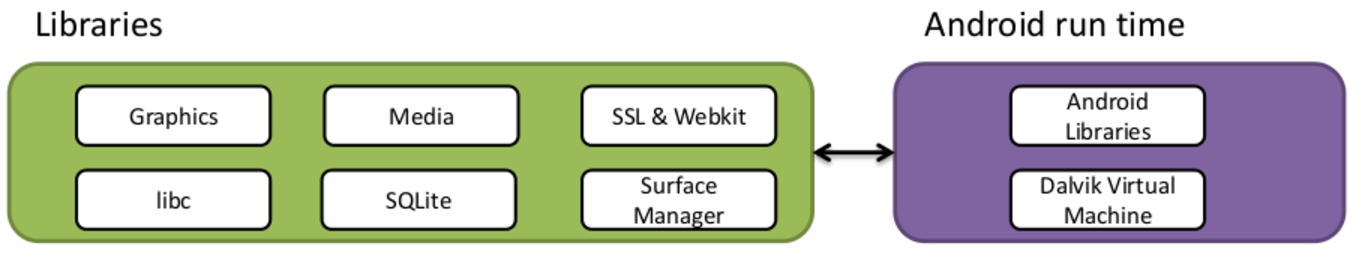
\includegraphics[width=\textwidth]{img/runtimeLibraries.pdf}
	\label{fig:kernel}
\end{figure}

\end{frame}

\begin{frame}
\frametitle{Run time}
\begin{itemize}
\item Core Libraries: proper implementations for the Dalvik Virtual Machine $\neq$ Java VM
\item Dalvik VM: virtual machine for Android, optimized for mobile devices (battery, processor \& memory management) 
\end{itemize}

\begin{figure}[b]
	\centering
		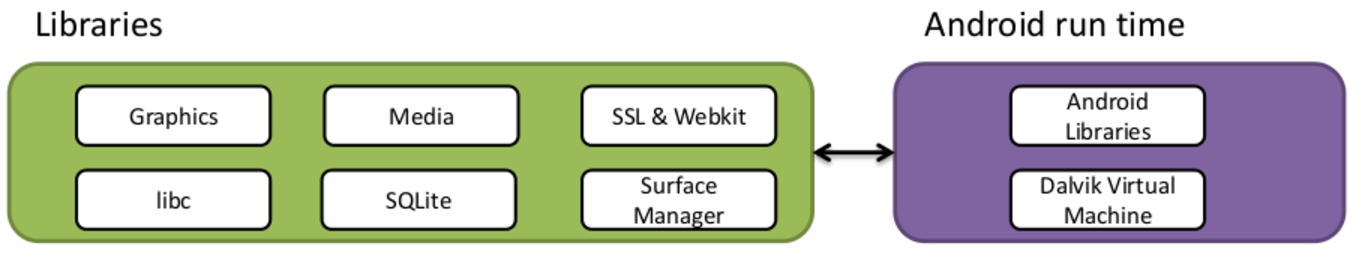
\includegraphics[width=\textwidth]{img/runtimeLibraries.pdf}
	\label{fig:kernel}
\end{figure}

\end{frame}

\begin{frame}
\frametitle{A typical work flow}

\begin{enumerate}
	\item App written in java
	\item compiled to Java bytecode files
	\item dx converts java bytecode files to a single dex bytecodefile (classes.dex)
	\item Dalvik executes dex bytecode file 
\end{enumerate}
\end{frame}

\begin{frame}
\frametitle{Application Framework}
	The application framework provides the classes which can be used to create Android applications: an interface for access to the hardware 
	\begin{figure}[b]
	\centering
		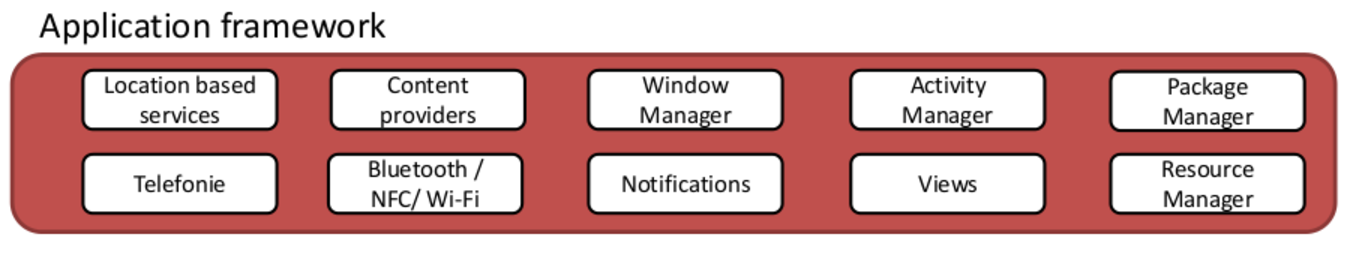
\includegraphics[width=\textwidth]{img/appFramework.pdf}
	\label{fig:kernel}
\end{figure}
\end{frame}

\begin{frame}
\frametitle{Application Layer}
	All applications are build in the application layer, using the different API libraries, and executed in the Dalvik VM. 
	\begin{figure}[b]
	\centering
		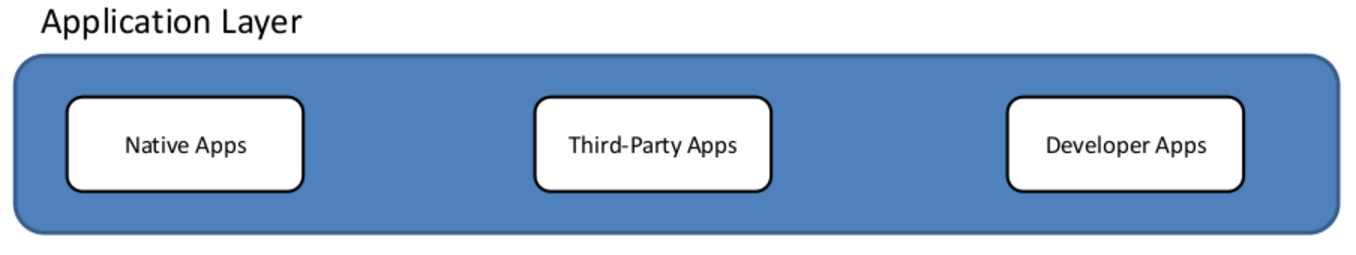
\includegraphics[width=\textwidth]{img/apllicationLayer.pdf}
	\label{fig:kernel}
\end{figure}
\end{frame}


{
	\usebackgroundtemplate{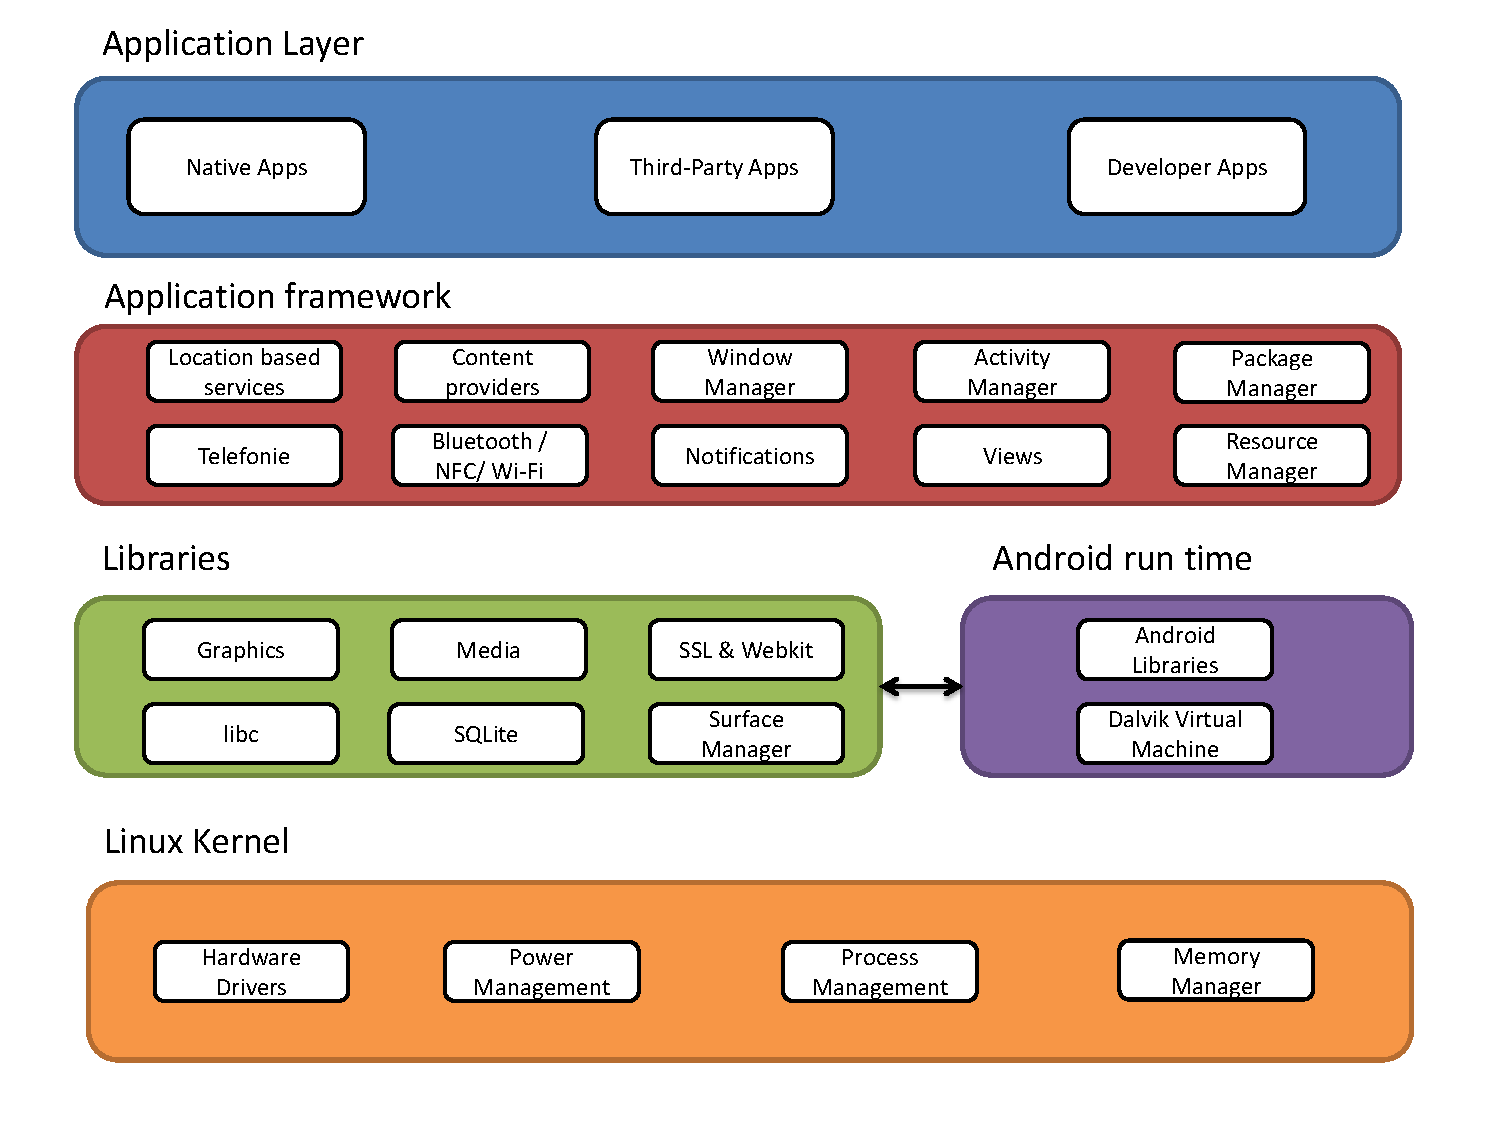
\includegraphics[height=\paperheight,width=\paperwidth]{img/androidstack.pdf}}
	\setbeamertemplate{navigation symbols}{}
	\begin{frame}[plain]
	\end{frame}
}




\section{Basic Programming in Android}
\sectionframe

\begin{frame}
\frametitle{Google is your friend!}
\begin{figure}
	\centering
		
\includegraphics[width=0.8\textwidth]{img/google.jpg}
	\label{fig:google}
\end{figure}
\end{frame}



\section{Activities \& Activity Lifecycle}
\sectionframe

\section{Tutorial: lets go for it!}
\sectionframe



%---------- Back matter -------------------------------------------------------

\end{document}
